\documentclass{article}
\usepackage[utf8]{inputenc}
\usepackage{amssymb}
\usepackage{cite}
\usepackage{subfig}
\usepackage{graphicx}
\usepackage{caption}
\usepackage{float}
\usepackage{amsmath}
\usepackage{listings}
\usepackage{xcolor}
\usepackage{inconsolata}
\usepackage{mdframed}
% \usepackage[portuguese]{babel}
\usepackage[document]{ragged2e}
\usepackage[letterpaper, margin=1.2in]{geometry}


\definecolor{light-gray}{gray}{0.9}

\lstset
{
    % frame=tb, % draw a frame at the top and bottom of the code block
    backgroundcolor = \color{light-gray},
    tabsize=4, % tab space width
    showstringspaces=false, % don't mark spaces in strings
    % numbers=left, % display line numbers on the left
    commentstyle=\color{gray}, % comment color
    keywordstyle=\color{blue}, % keyword color
    stringstyle=\color{red}, % string color
    basicstyle=\footnotesize\ttfamily,
    breaklines=true,
    language=C++,
    literate=   % letters not supported
      {á}{{\'a}}1 {é}{{\'e}}1 {í}{{\'i}}1 {ó}{{\'o}}1 {ú}{{\'u}}1
      {Á}{{\'A}}1 {É}{{\'E}}1 {Í}{{\'I}}1 {Ó}{{\'O}}1 {Ú}{{\'U}}1
      {à}{{\`a}}1 {è}{{\`e}}1 {ì}{{\`i}}1 {ò}{{\`o}}1 {ù}{{\`u}}1
      {À}{{\`A}}1 {È}{{\'E}}1 {Ì}{{\`I}}1 {Ò}{{\`O}}1 {Ù}{{\`U}}1
      {ä}{{\"a}}1 {ë}{{\"e}}1 {ï}{{\"i}}1 {ö}{{\"o}}1 {ü}{{\"u}}1
      {Ä}{{\"A}}1 {Ë}{{\"E}}1 {Ï}{{\"I}}1 {Ö}{{\"O}}1 {Ü}{{\"U}}1
      {â}{{\^a}}1 {ê}{{\^e}}1 {î}{{\^i}}1 {ô}{{\^o}}1 {û}{{\^u}}1
      {Â}{{\^A}}1 {Ê}{{\^E}}1 {Î}{{\^I}}1 {Ô}{{\^O}}1 {Û}{{\^U}}1
      {œ}{{\oe}}1 {Œ}{{\OE}}1 {æ}{{\ae}}1 {Æ}{{\AE}}1 {ß}{{\ss}}1
      {ű}{{\H{u}}}1 {Ű}{{\H{U}}}1 {ő}{{\H{o}}}1 {Ő}{{\H{O}}}1
      {ç}{{\c c}}1 {Ç}{{\c C}}1 {ø}{{\o}}1 {å}{{\r a}}1 {Å}{{\r A}}1
      {€}{{\euro}}1 {£}{{\pounds}}1 {«}{{\guillemotleft}}1
      {»}{{\guillemotright}}1 {ñ}{{\~n}}1 {Ñ}{{\~N}}1 {¿}{{?`}}1
      {ã}{{\~a}}1 {õ}{{\~o}}1 {∆}{{\tiny$\Delta$}}1
      {^}{{\^{}}}1 {±}{{$\pm$}}1
}

\lstnewenvironment{code}[1][C++]
{%
    \mdframed
        [
        backgroundcolor=light-gray, roundcorner=10pt,leftmargin=1, rightmargin=1, innerleftmargin=5, innertopmargin=5,innerbottommargin=5, outerlinewidth=1, linecolor=light-gray
        ]%
    \lstset{
        language=#1
    }
}
{
    \endmdframed
}

\title{Robotic Arm Continuous Control Project}
\author{Tiago Montalvão}

\begin{document}

\maketitle
\justify

\section{Introduction}

This is a report of the second project of Udacity Deep Reinforcement Learning Nanodegree. It describes the model architecture with chosen hyperparameters used in the agent, the experiments, and potential improvements upon the current results.

The environment chosen in this project is the second one provided, in which there are 20 multiple arms interacting with the world simultaneously.

\section{Implementation}
\subsection{Agent}

The agent was implemented using Deep Deterministic Policy Gradient (DDPG). This algorithm is basically an enhancement of Deep Q-Networks (DQN) for dealing not only with a continuous state space but also with a continuous action space.

It is categorized as an Actor-Critic method, because there are two networks (Actor and Critic) collaborating to achieve the agents' results. Basically, the actor learns to pick actions from states, while the critic learns to calculate the state-action Q value function.

The DDPG was then implemented with:

\begin{itemize}
    \item \textbf{Experience replay buffer} to handle data correlation between consecutive samples.
    \item \textbf{Two neural networks} with identical architecture (local and target networks) for each actor and critic, as described in the following section (so there were 4 networks in total). \textbf{Soft update} was also implemented to updated each target network, instead of updating the whole network every n-th iteration.
    \item \textbf{Ornstein–Uhlenbeck process} implemented to add noise to the actions, thus creating incentives to exploration. 
\end{itemize}

It is worth mentioning that the implementation was heavily based on previously implemented DDPG on the Nanodegree, but a few adjustments were made in the hyperparameters and in the code itself. The adjustments were:

\begin{itemize}
    \item Ornstein–Uhlenbeck process fixed to sample from Standard Normal distribution instead of [0, 1) uniform distribution.
    \item Replay buffer support for adding multiple samples (one for each agente) at once.
    \item Gradient clipping in the critic network update.
    \item Instead of sampling from the replay buffer and learning from these tuples every iteration, a counter was implemented to only update the network each UPDATE\_EVERY iterations.
    \item Each UPDATE\_EVERY iterations, tuples were sampled and the networks were updated a few times in a row (N\_UPDATES\_PER\_STEP hyperparameter).
    \item The batch size of samples from the replay buffer was significantly increased from 128 to 1024. Before that, the learning was quite slow (environment solved in more than 400 episodes).
\end{itemize}

These adjustments gave a lot of stability for the learning process.

The chosen hyperparametes are described above:

\begin{code}[Python]
BUFFER_SIZE = int(1e6)    # replay buffer size
BATCH_SIZE = 1024         # minibatch size
GAMMA = 0.975             # discount factor
TAU = 1e-3                # for soft update of target parameters
LR_ACTOR = 5e-4           # learning rate of the actor 
LR_CRITIC = 1e-3          # learning rate of the critic
WEIGHT_DECAY = 0          # L2 weight decay
UPDATE_EVERY = 15         # how often to update the network
N_UPDATES_PER_STEP = 10   # number of updates to perform at each learning step
\end{code}

\subsection{Model architecture}

The architecture for the actor network is as follows:

\begin{figure}[H]
\centering
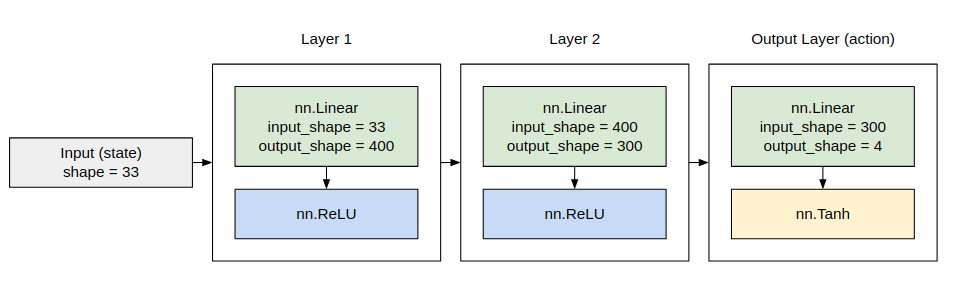
\includegraphics[scale=0.45]{img/actor_arch.png}
\label{fig:actor_arch}
\end{figure}

The architecture for the actor network is as follows:

\begin{figure}[H]
\centering
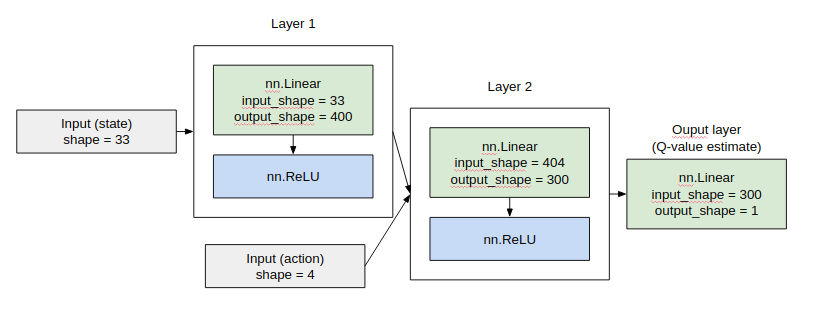
\includegraphics[scale=0.45]{img/critic_arch.png}
\label{fig:critic_arch}
\end{figure}

In the project notebook, there is a cell which executes a command that gives the model summary (the same info above with some numbers). Based on this, we can get the information that there are 135104 trainable parameters in the actor network and 135401 trainable parameters in the critic network.

\section{Results}

The agent was able to solve the environment in only 102 episodes, and it took it about 70 minutes to train. All the details can be checked in the project notebook. It can be seen that the agent could learn quite well in early episodes and in a very stable way.

The following image shows the individual episode score (in blue),the moving average of the last 100 episodes' scores (in orange), and the threshold of 30 for the moving average (in red), so that the environment is considered solved.

\begin{figure}[H]
\centering
\centering
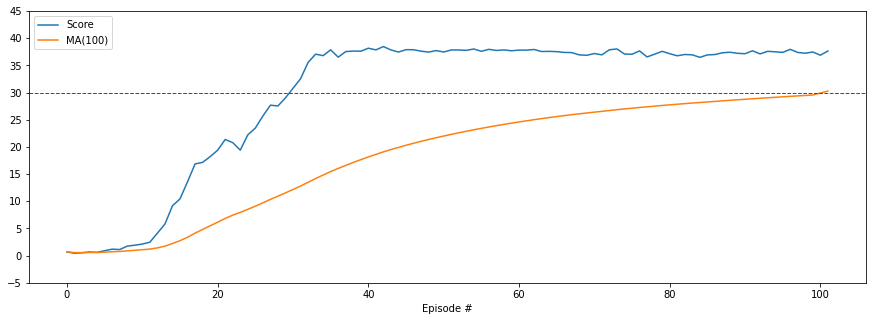
\includegraphics[scale=0.5]{img/score.png}
\label{fig:score}
\end{figure}

\section{Ideas for Future Work}

DDPG is one of the most classic actor-critic algorithms. Other algorithms (like PPO, TRPO, A3C, D4PG) could be implemented for practicing purposes because the results obtained were satisfactory (maybe other algorithms could speed up training process).

Another improvement could be the addition of \textbf{Prioritized Experience Replay}, giving more weight in experience sampling from replay buffer for tuples that have larger TD errors.

\end{document}
